\section{DIS pseudo-data generation}
\label{sec:dis_pseudodata}

Here we describe the procedure adopted in order 
to generate projections for the kinematic coverage
and experimental uncertainties associated to differential measurements
of neutrino-nucleus scattering at the LHC far-forward experiments.
%
First, we summarise the theoretical description of differential
neutrino scattering in terms of DIS structure functions and highlight
their PDF sensitivity.
%
Second, we present an  overview of the operative and proposed
LHC far-forward neutrino detectors that
will be considered in the present study and indicate their
key acceptance and performance parameters.
%
By convoluting the expected muon neutrino fluxes
with the acceptance and scattering rates of each
of these detectors,
we compute the foreseen event yields in bins of $x$, $Q^2$,
and $E_\nu$ and therefore the associated statistical uncertainties.
%
Finally, we estimate how the dominant systematic
uncertainties in each experiment translate into uncertainties in the predicted
event rates and use this information to complete the calculation of the experimental
covariance matrix.

\subsection{Neutrino DIS revisited}

The double-differential cross-section for neutrino-nucleus charged-current scattering,
see~\cite{Candido:2023utz} and references therein,
can be expressed in terms of 
independent structure functions $F_2^{\nu A}$, $xF_3^{\nu A}$
and $F_L^{\nu A}$:
\be
\label{eq:neutrino_DIS_xsec_FL}
\frac{d^2\sigma^{\nu A}(x,Q^2,y)}{dxdy} =  \frac{G_F^2s/4\pi}{\lp 1+Q^2/m_W^2\rp^2}\lc Y_+F^{\nu A}_2(x,Q^2) - y^2F^{\nu A}_L(x,Q^2) +Y_- xF^{\nu A}_3(x,Q^2)\rc  \, ,
\ee
where $Y_\pm = 1 \pm (1-y)^2$ and with a counterpart expression for anti-neutrino scattering,
\be
\label{eq:antineutrino_DIS_xsec_FL}
\frac{d^2\sigma^{\bar{\nu} A}(x,Q^2,y)}{dxdy} =  \frac{G_F^2s/4\pi}{\lp 1+Q^2/m_W^2\rp^2}\lc Y_+F^{\bar{\nu} A}_2(x,Q^2) - y^2F^{\bar{\nu} A}_L(x,Q^2) -Y_- xF^{\bar{\nu} A}_3(x,Q^2)\rc  \, ,
\ee
where $s=2m_N E_\nu$ being the neutrino-nucleon center of mass energy squared, $m_N$ is the nucleon mass,
$E_\nu$ is the incoming neutrino energy,
and the inelasticity is $y=Q^2/(2x m_n E_{\nu})$.
%
Structure functions depend only on $x$ and $Q^2$ while the differential
cross-section depends also on the neutrino energy $E_\nu$, or alternatively
on the inelasticity $y$.
%
Further, structure functions $F^{\nu A}_i(x,Q^2)$ and $F^{\bar{\nu} A}_i(x,Q^2)$ depend on the nuclear target $A$ entering
for the neutrino scattering through the nuclear modifications of the proton PDFs.

Eqns.~(\ref{eq:neutrino_DIS_xsec_FL}) and~(\ref{eq:antineutrino_DIS_xsec_FL}) are valid provided
the hadronic 
invariant mass $W$  is above the resonance threshold,
\be
W^2 = \lp m_N^2 + Q^2 \frac{(1-x)}{x} \rp \gsim \lp 2\,{\rm GeV} \rp^2\, ,
\ee
and in addition here we  restrict ourselves to the DIS region with perturbative momentum
transfers $Q^2$, such that
 structure functions are decomposed as
\be
\label{eq:sfs_pqcd}
 F^{\nu A}_i(x,Q^2) = \sum_{j=q,\bar{q},g}\int_x^1 \frac{dz}{z}\, C_{i,j}^{\nu N}(z,\alpha_s(Q^2))f^{(A)}_j\lp \frac{x}{z},Q^2\rp \, , \quad i = 2,3,L \, .
 \ee
%
in terms of a convolution of partonic scattering cross-sections  $C_{i,j}^{\nu N}(x,\alpha_s)$ and
of process-independent PDFs $f^{(A)}_j\lp x,Q^2\rp$.
%
A similar expression holds for charm production~\cite{Faura:2020oom}, which requires
accounting also for charm mass effects~\cite{Gao:2017kkx}.
 %
We discuss in Sect.~\ref{sec:settings} the theoretical
settings adopted~\cite{Candido:2022tld,yadism,Candido:2023utz,Carrazza:2020gss} to
evaluate predictions for
neutrino DIS structure functions, Eq.~(\ref{eq:sfs_pqcd}),
and for differential cross-sections,
Eqns.~(\ref{eq:neutrino_DIS_xsec_FL}) and~(\ref{eq:antineutrino_DIS_xsec_FL}),
in the kinematic range of relevance for LHC neutrinos.

 Each neutrino structure function provides complementary sensitivity
 to the partonic flavour decompositions of nucleons.
 %
 To illustrate this sensitivity, consider a leading order  calculation
 for a proton target with $n_f=4$ active quark flavours,
a diagonal CKM matrix and no heavy quark mass effects.
 %
 The resulting $F_2^{\nu p}$ and $xF_3^{\nu p}$ structure functions read
 \bea
 F_2^{\nu p}(x,Q^2) &=& 2x\lp f_{\bar{u}} + f_{d} + f_{s} + f_{\bar{c}} \rp(x,Q^2) \, , \nonumber  \\
 F_2^{\bar{\nu} p}(x,Q^2) &=& 2x\lp f_u + f_{\bar{d}} + f_{\bar{s}} + f_c \rp(x,Q^2) \, , \label{eq:neutrinoSFs_proton} \\
 xF_3^{\nu p}(x,Q^2) &=& 2x\lp -f_{\bar{u}} + f_d +f_s - f_{\bar{c}}\rp(x,Q^2)  \, , \nonumber\\
 xF_3^{\bar{\nu} p}(x,Q^2) &=& 2x\lp f_u - f_{\bar{d}} -f_{\bar{s}} + f_{c}\rp(x,Q^2) \, . \nonumber
 \eea
 The corresponding expressions for a neutron target are obtained from isospin symmetry
 \bea
 F_2^{\nu n}(x,Q^2) &=& 2x\lp f_{\bar{d}} + f_{u} + f_{s} + f_{\bar{c}} \rp(x,Q^2) \, , \nonumber  \\
 F_2^{\bar{\nu} n}(x,Q^2) &=& 2x\lp f_d + f_{\bar{u}} + f_{\bar{s}} + f_c \rp(x,Q^2) \, , \label{eq:antineutrinoSFs_neutron} \\
 xF_3^{\nu n}(x,Q^2) &=& 2x\lp -f_{\bar{d}} + f_u +f_s - f_{\bar{c}}\rp(x,Q^2)  \, , \nonumber\\
 xF_3^{\bar{\nu} n}(x,Q^2) &=& 2x\lp f_d - f_{\bar{u}} -f_{\bar{s}} + f_{c}\rp(x,Q^2) \, , \nonumber
 \eea
 while for an isoscalar, free-nucleon target denoted by $N$ one has
 \bea
 F_2^{\nu N}(x,Q^2) &=& 2x\lp f_{u^+} + f_{d^+} + 2f_s + 2f_{\bar{c}} \rp(x,Q^2) \, , \nonumber  \\
 F_2^{\bar{\nu} N}(x,Q^2) &=& 2x\lp f_{u^+} + f_{d^+} + 2f_{\bar{s}} + 2f_c \rp(x,Q^2) \, , \label{eq:neutrinoSFs_isoscalar} \\
 xF_3^{\nu N}(x,Q^2) &=& 2x\lp f_{u^-} + f_{d^-} +2f_s - 2f_{\bar{c}}\rp(x,Q^2)  \, , \nonumber\\
 xF_3^{\bar{\nu} N}(x,Q^2) &=& 2x\lp   f_{u^-} + f_{d^-}-2f_{\bar{s}} +2 f_{c}\rp(x,Q^2) \, , \nonumber
 \eea
 in terms of the valence and sea PDF combinations defined by
 \be
 f_{q^+} (x,Q^2)\equiv \lp f_{q}+f_{\bar{q}}\rp(x,Q^2) \, , \qquad
 f_{q^-} (x,Q^2)\equiv \lp f_{q}- f_{\bar{q}}\rp(x,Q^2) \, .
 \ee
 We note that even for isoscalar targets separate measurements
 for neutrinos and antineutrinos will not be equivalent, since in general neither $f_{s^-}$ nor
 $f_{c^-}$ are expected to vanish.

 In the projections presented in this work, when interpreting the LHC neutrino structure
 functions in terms of proton PDFs we will assume a isoscalar free-nucleon target and neglect
 nuclear PDF modifications, along the lines of Eq.~(\ref{eq:neutrinoSFs_isoscalar}).
 %
 On the other hand, when evaluating structure functions
 for a tungsten (W) target, we keep into account both
 nuclear corrections and that
 the target is not isoscalar when evaluating the physical observables.
 %
 We point out that accounting for nuclear target effects in a global proton
 PDF fit is straightforward by means of the procedure developed
 in~\cite{Ball:2020xqw,Ball:2018twp}.

 It is illustrative to compare the PDF dependence of neutrino structure functions
 at LO with that of their counterparts for neutral-current
 scattering with a charged lepton projectile.
 %
 Within the same assumptions, for energies below
 the $Z$-boson mass, $Q^2 \ll m_Z$, the corresponding
 partonic decomposition is
 the 
 \bea
 F_2^{\ell p}(x,Q^2) &=& x\lp \frac{4}{9}\lc f_{u^+} + f_{c^+}\rc
 + \frac{1}{9}\lc f_{d^+} + f_{s^+}\rc\rp(x,Q^2) \, , \nonumber  \\
 F_2^{\ell n}(x,Q^2) &=& x\lp \frac{4}{9}\lc f_{d^+} + f_{c^+}\rc
 + \frac{1}{9}\lc f_{u^+} + f_{s^+}\rc\rp(x,Q^2) \, ,\label{eq:NC_chargedlepton}   \\
 F_2^{\ell N}(x,Q^2) &=& x\lp \frac{5}{18}\lc f_{u^+} + f_{d^+}\rc
 + \frac{1}{9} f_{s^+} + \frac{4}{9} f_{c^+} \rp(x,Q^2) \, , \nonumber  
 \eea
 with $xF_3$ being negligible in this region.
 %
 Eq.~(\ref{eq:NC_chargedlepton}) showcases the complementarity between
 neutrino and charged-lepton DIS in terms of sensitivity
 to the flavour PDF decomposition.

 \subsection{Far-forward neutrino detectors at the LHC}
 \label{sec:neutrinoDetectors}

 As we discuss below, the calculation of differential neutrino scattering event rates
 at the LHC far-forward detectors requires two main ingredients: the energy
 and flavour dependence of the incoming neutrino flux crossing
 the detector fiducial volume, on the one hand,
 and the scattering rates within the same fiducial volume, on the other hand.
 %
 In this section, we summarise the main features of each of the ongoing and future
 far-forward detectors considered in this study, in particular concerning
 their acceptance, geometry, and neutrino detection method.
 %
 We also indicate the expected performance of the three FPF detectors
 and how this translates into the dominant experimental systematic
 uncertainties.
 %
 Since for the projection studies considered in this work we focus on muon
 neutrino scattering, we will focus the subsequent discussion on the detection
 performance of this neutrino flavour.

 Table~\ref{tab:FPF_experiments} indicates
 the rapidity coverage, target material,
 muon neutrino acceptance, and the identification and reconstruction performance
 for each of the far-forward LHC neutrino experiments considered
 in this work.
 %
 More details of the information listed in this table is provided
 in the following.

  %-----------------------------------------------------------------
\begin{table}[h!]
  \centering
  \small
  \renewcommand{\arraystretch}{1.60}
\begin{tabularx}{\textwidth}{Xcccc}
\toprule
Detector &  Rapidity &  Target &  Acceptance  & Performance \\
\midrule
FASER$\nu$  &   &     &       &              \\
SND@LHC  &   &     &       &              \\
\midrule
FASER$\nu$2  &   &     &       &              \\
AdvSND  &   &     &       &              \\
FLArE  &   &     &       &              \\
  \bottomrule
\end{tabularx}
\vspace{0.2cm}
\caption{\small For each of the far-forward LHC neutrino experiments considered
  in this work we indicate their rapidity coverage, target material,
  muon neutrino acceptance, and the identification and reconstruction performance.
  \label{tab:FPF_experiments}
}
\end{table}
%-----------------------------------------------------------------
 

 \paragraph{AdvSND.}
 %
 The AdvSND far-detector will be able to track muons with energy $E_\nu \gsim 20$ GeV
 within an acceptance of 100 mrad with information on the charge
 of the  outgoing charged leptons.
 %
 The total energy of the hadronic final state can also be measured.
 %
 A proposed ``near-detector'' companion is being discussed for AdvSND, but
 it would not be installed in the FPF and hence is not discussed here further.

 \paragraph{FLArE.}
 %
 A liquid argon (LAr) detector able to track muon neutrinos
 with energies  $E\le 1.5~\rm{TeV}$ with
 a scattering angle reaching up to 0.4 mrad.
 %
 No information on the sign of the charged leptons can be extracted.
 %
 Reconstruction of the total energy of the hadronic final state should be
 possible. 
 %
 A $\delta E_\nu\sim$30\% of energy resolution is
 the target performance for muons, with an associated
 $\delta \sim 5$ mrad of angular  resolution.

 % Table coverage + detector performance




 

\subsection{Differential event rate calculation}
\label{sec:pseudo-data_generation}

The first goal is to produce projections
for DIS pseudo-data at the FPF based on
some idealised detector concepts and
some initial choice of neutrino fluxes
e.g.~\cite{Kling:2021gos}.
%
This requires a knowledge of the detector geometry
and material, as well as of the double-differential
neutrino interaction cross-section. 
%
Since we aim to produce pseudo-data binned in $(x,Q^2)$,
for each simulated event we need to determine the 
final-state kinematics. 

Specifically, we would like to evaluate the
number of charged-current neutrino interaction events
within the detector volume in different bins
of the incoming neutrino energy $E_\nu$, the Bjorken
variable $x$ and the momentum transfer square $Q^2$,
\begin{equation}
    N_{\rm ev}(E_\nu, x, Q^2) \, ,
\end{equation}
for some binning in these three kinematic variables.
%
This can be evaluated as
\begin{equation}
\label{eq:nev_v1}
    N_{\rm ev}(E_\nu, x, Q^2) \propto \int_{\rm bin}\int_{\rm det}  \frac{d^2\sigma^{\nu A}(x,Q^2,y)}{dxdy} \mathcal{L}_{\nu}(E_{\nu}) \, ,
\end{equation}
where $\mathcal{L}(E_{\nu}) $ is the incoming neutrino
luminosity which accounts for the detector geometry
and material density. 
%
Eq.~(\ref{eq:nev_v1}) can be integrated to
determine the actual number of events within
the bin boundaries.

We start with a perfect detector.


For bins in $x,Q^2,E_{\nu}$, we start with the \href{https://github.com/juanrojochacon/FPF-WG1/blob/main/results/diff_xsecs_a1.txt}{differential cross section},$\frac{d^2\sigma(x,Q^2,E_{\nu}}{dxdQ^2})$ [pb GeV$^{-2}$] as output from {\tt YADISM} and convolve with the \href{https://github.com/KlingFelix/FastNeutrinoFluxSimulation/tree/main/Fluxes}{neutrino flux}, $\frac{dN_{\nu}}{dE_{\nu}}$. So for a detector with $n_T$ nuclear target density and $L_T$ length, we calculate the event rate per bin as

\begin{equation}
    N_{\rm ev}/{\rm bin} = n_T L_T\int_{Q^2_{min}}^{Q^2_{max}}\int_{x_{min}}^{x_{max}}\int_{E_{\nu,min}}^{E_{\nu , max}} \frac{dN_{\nu}}{dE_{\nu}}\left(\frac{d^2\sigma(x,Q^2,E_{\nu})}{dxdQ^2}\right) dQ^2 dx dE_{\nu}.
\end{equation}

Using a MC integration, we can calculate $N_{\rm ev}/{\rm bin}$ by sampling $N$ points in $x,Q^2,E_{\nu}$ space such that $0< y = \frac{Q^2}{2m_N E_{\nu }x} < 1$ and integrating over the bin.

\begin{equation}
    N_{\rm ev}/{\rm bin} \approx n_T L_T \frac{(Q^2_{max}-Q^2_{min})(x_{max}-x_{min})(E_{\nu ,max}-E_{\nu ,min})}{N}\times \sum_i^N f(x_i,Q^2_i,E_{\nu ,i})
    \label{MCintegration}
\end{equation}

where $f(x_i,Q^2_i,E_{\nu ,i}) = \frac{dN_{\nu}}{dE_{\nu,i}}\left(\frac{d^2\sigma(x_i,Q^2_i,E_{\nu,i})}{dxdQ^2}\right)$. 

The statistical uncertainty for each bin is then defined by a Gaussian distribution with fractional uncertainty $1/\sqrt{N{\rm ev}/{\rm bin}}$, i.e. $\delta N_{\rm ev}/{\rm bin} = \sqrt{N_{\rm ev}} /{\rm bin}$


  Following this prescription, we can produce plots which characterize the event rate for a particular neutrino species at a particular experiment. 

Results for FASER$\nu$2 can be found \href{https://github.com/juanrojochacon/FPF-WG1/tree/main/results}{here}. The .txt files will display which neutrino species was considered, and also compile experimental geometries and target details in the header. In the sub-folder \href{https://github.com/juanrojochacon/FPF-WG1/tree/main/results/Summaries}{summaries}, plots can be found which show the event rate in $x,Q^2$ space, integrating over the entire neutrino spectrum. The event rate for muon neutrinos at FASER$\nu$2 is shown in Fig~\ref{fig:fasernu2_muon}.

\begin{figure}[h]
    \centering
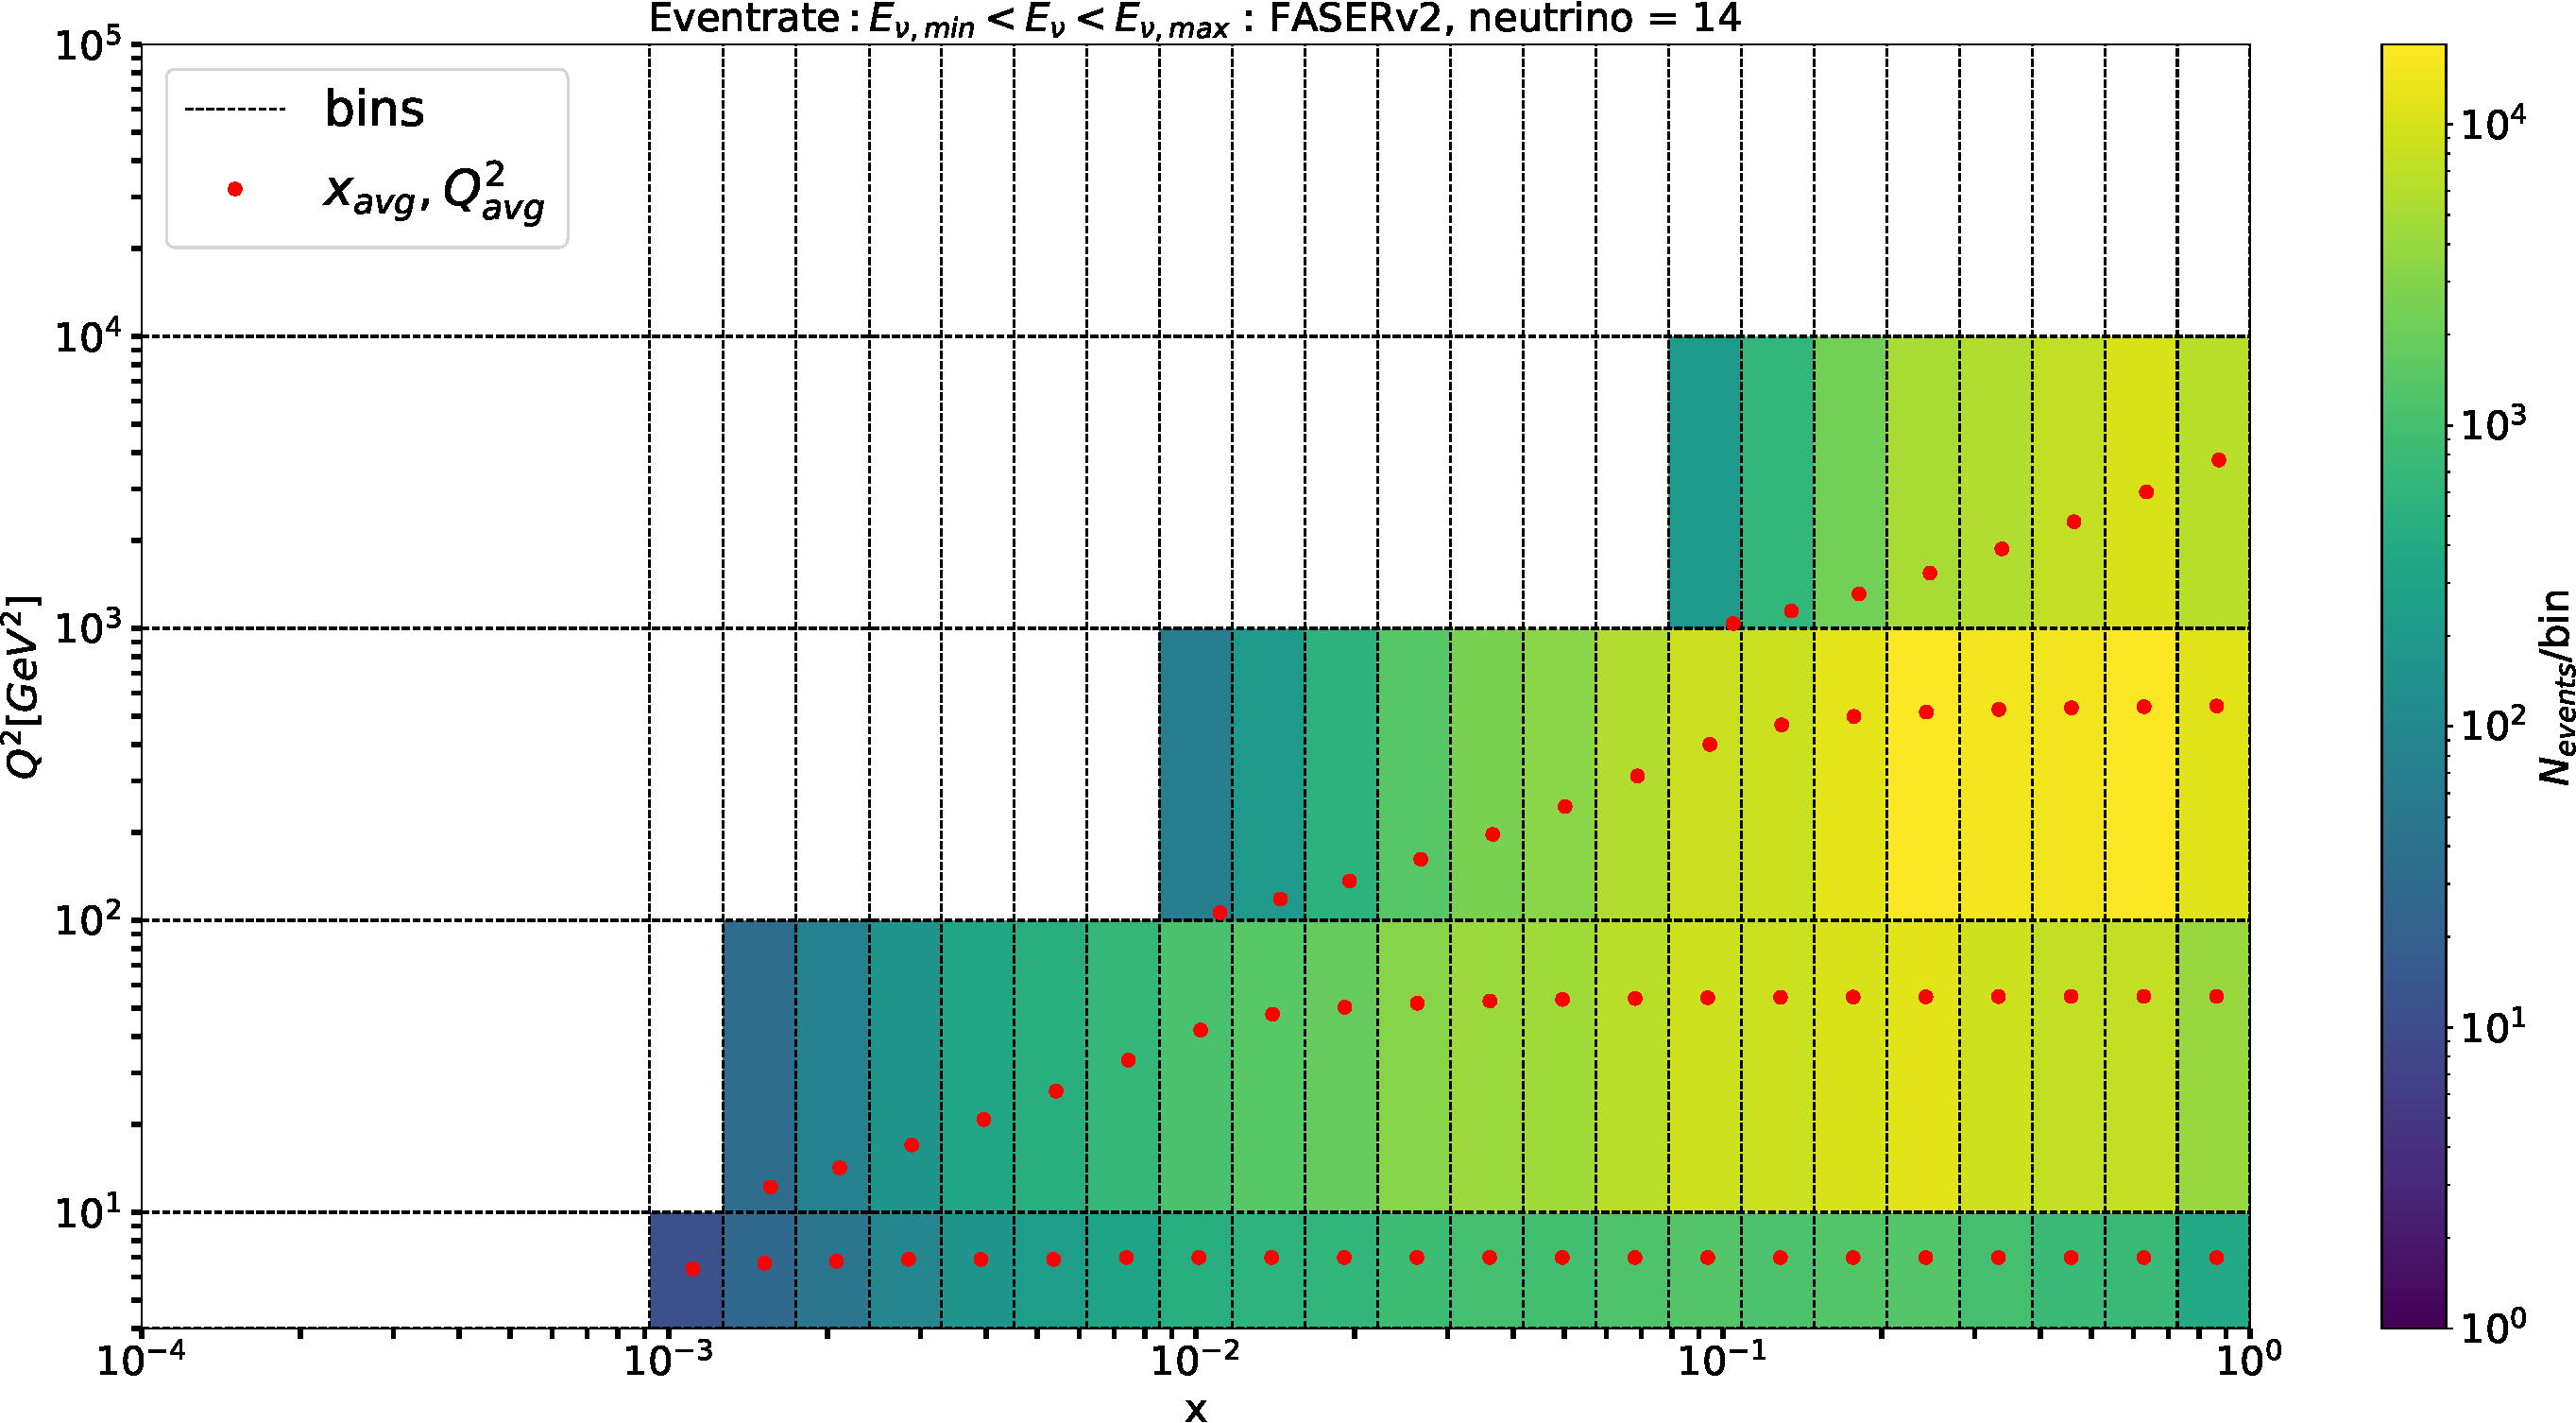
\includegraphics[width=1\textwidth]{plots/Nevent_FASERv2_14.pdf}
    \caption{Event rate per bin for muon neutrinos at FASER$\nu$2. Bins are denoted by dashed grid, and the red dot indicates the weighted average of $x,Q^2$ points in each bin. The total number of muon neutrino events calculated is $\approx2.6\times 10^5$. Note that bins were chosen somewhat arbitrarily, and can be iterated to improve PDF fits }
    \label{fig:fasernu2_muon}
\end{figure}

\subsection{Estimating systematic uncertainties}

We now wish to understand the impact of systematic uncertainties on the event rate in $(x,Q^2,E_{\nu})$ space. For each experiment, the observables $E_{l},E_{h},\theta$ are related to $(x,Q^2,E_{\nu})$ by 

\begin{align}
E_{\nu} = E_l + E_h \nonumber \\
Q^2 = 4E_lE_{\nu}\sin^2{\theta/2} \nonumber \\
x = \frac{Q^2}{2m_N(E_{\nu} - E_l)}.
\end{align}

We wish to sample over the space of observables, $(E_{l},E_{h},\theta)$, perform  cuts based on detector performance, calculate the event rates, and then smear this sampling according to experimental uncertainties to estimate the uncertainty on the event rate. 

Taking FASER${\nu}$2 as an example, we can write the experimental cuts and uncertainties as 

\begin{align}
100 < E_l < E_{\nu,{\rm max}} , \delta E_l = 30\% \nonumber \\
100 < E_h < E_{\nu,{\rm max}} , \delta E_h = 50\% \nonumber \\
0 < \theta < \tan^{-1}(0.5) , \delta\theta = 1~{\rm mrad}
\label{fasernu2systematic_errors}
\end{align}

We first generate a MC dataset, $D_0$, over this space with $N = 10^7$ samples and calculate $x,Q^2,E_{\nu}$ for each event, removing samples with $y > 1$. We then integrate according to Eq. \ref{MCintegration} to produce a distribution of events with bins in $x,Q^2,E_{\nu}$. We then smear each sample according to a Gaussian distribution with widths given by Eq.~\ref{fasernu2systematic_errors} to produce a new data set $D_i$ and repeat to produce $M = 10$ event distributions($M>10$ can later be used, but $M = 10$ appears to be stable). For each bin we take the standard deviation to produce the systematic errors per bin (denoted as "N\textunderscore sys\textunderscore errs" in files named "binned\textunderscore sys-events... .txt" \href{https://github.com/juanrojochacon/FPF-WG1/tree/main/results}{here}). 

For FASER${\nu}$2, the systematic errors typically dominate over statistical errors, at about $10\%$. 

\begin{figure}[h]
    \centering
    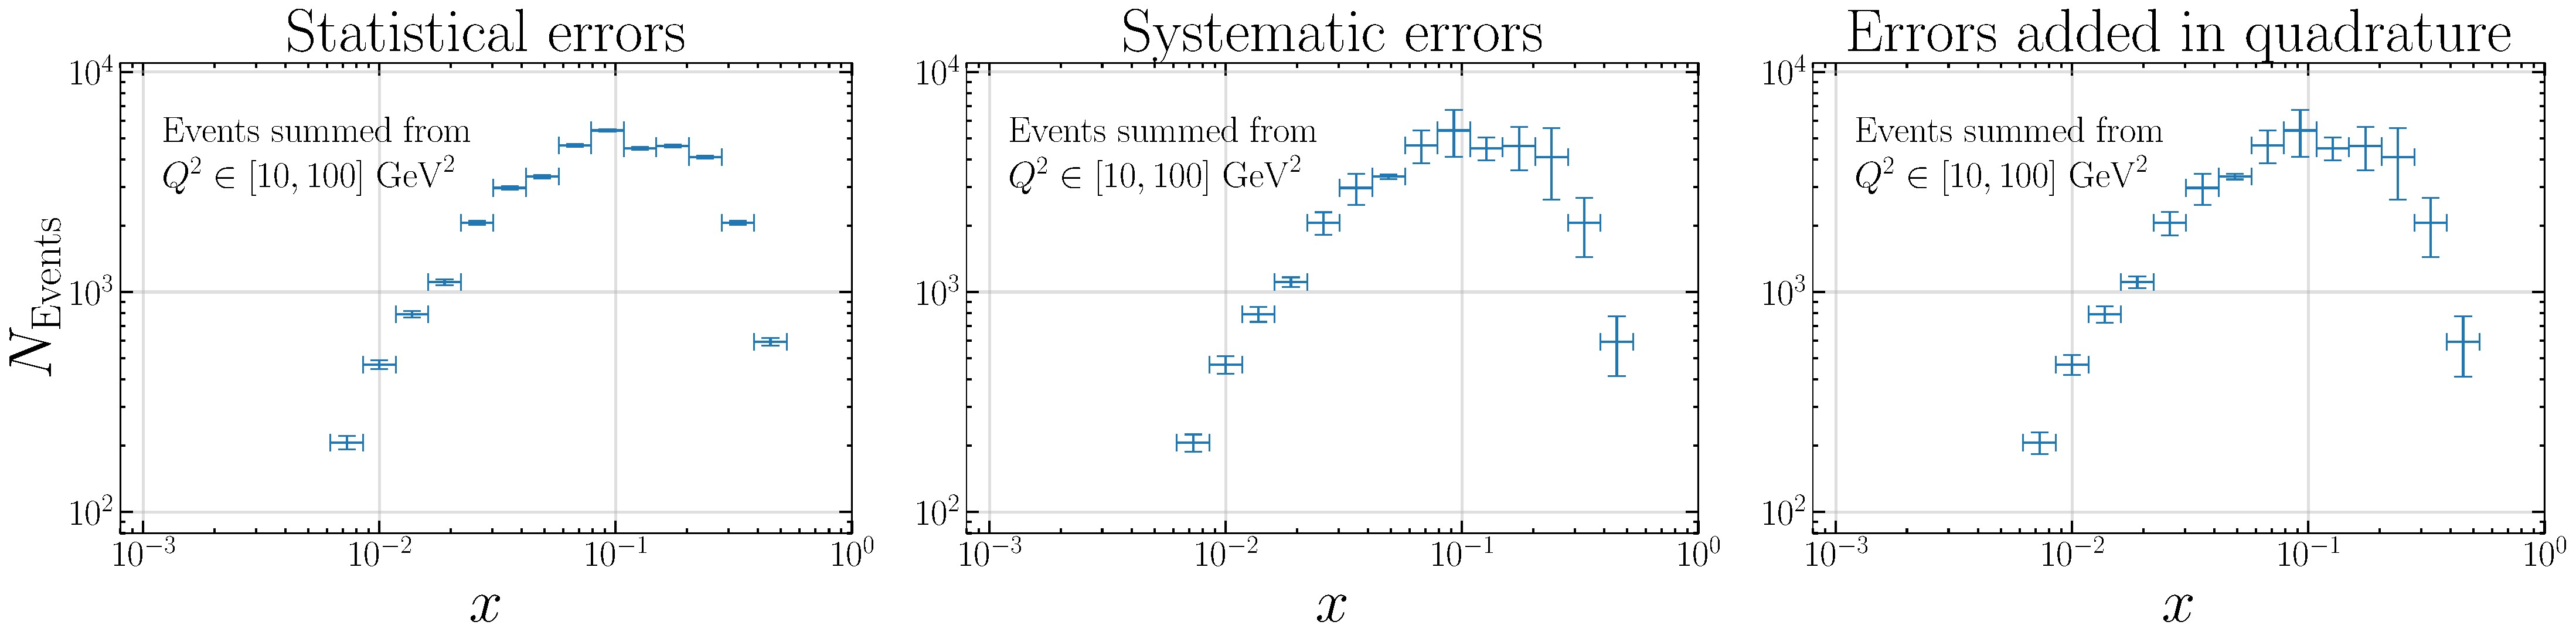
\includegraphics[width = 1\textwidth]{plots/error_plot_FASERv2_14.pdf}
    \caption{Event rates with error bars at FASER$\nu$2 for $\nu_{\mu} N \rightarrow \mu^- X$} summed over $Q^2$. The error bars along the x-axis showing the width of the $x$-bins, and are not showing any type of error.
    \label{fig:my_label}
\end{figure}

